\chapter{Preclinical Imaging}


Preclinical Molecular Imaging, Fig.\ref{fig:preclincal-imaging}, using microPET
(Sect.\ref{sec:microPET}), microCT (Sect.\ref{sec:microCT}) and Optical Methods.
\begin{itemize}
  
  \item  Optical fluorescent signal is linked to the growth factor, thus optical
  images show drug delivery over time.

  \item CT images show bone growth over time 
\end{itemize}
They provide complementary information,
Fig.\ref{fig:preclincal-imaging-pros-cons}. However, the output of each method
depends upon different conditions, Fig.\ref{fig:preclincal-imaging-depend}.

\begin{figure}[hbt]
  \centerline{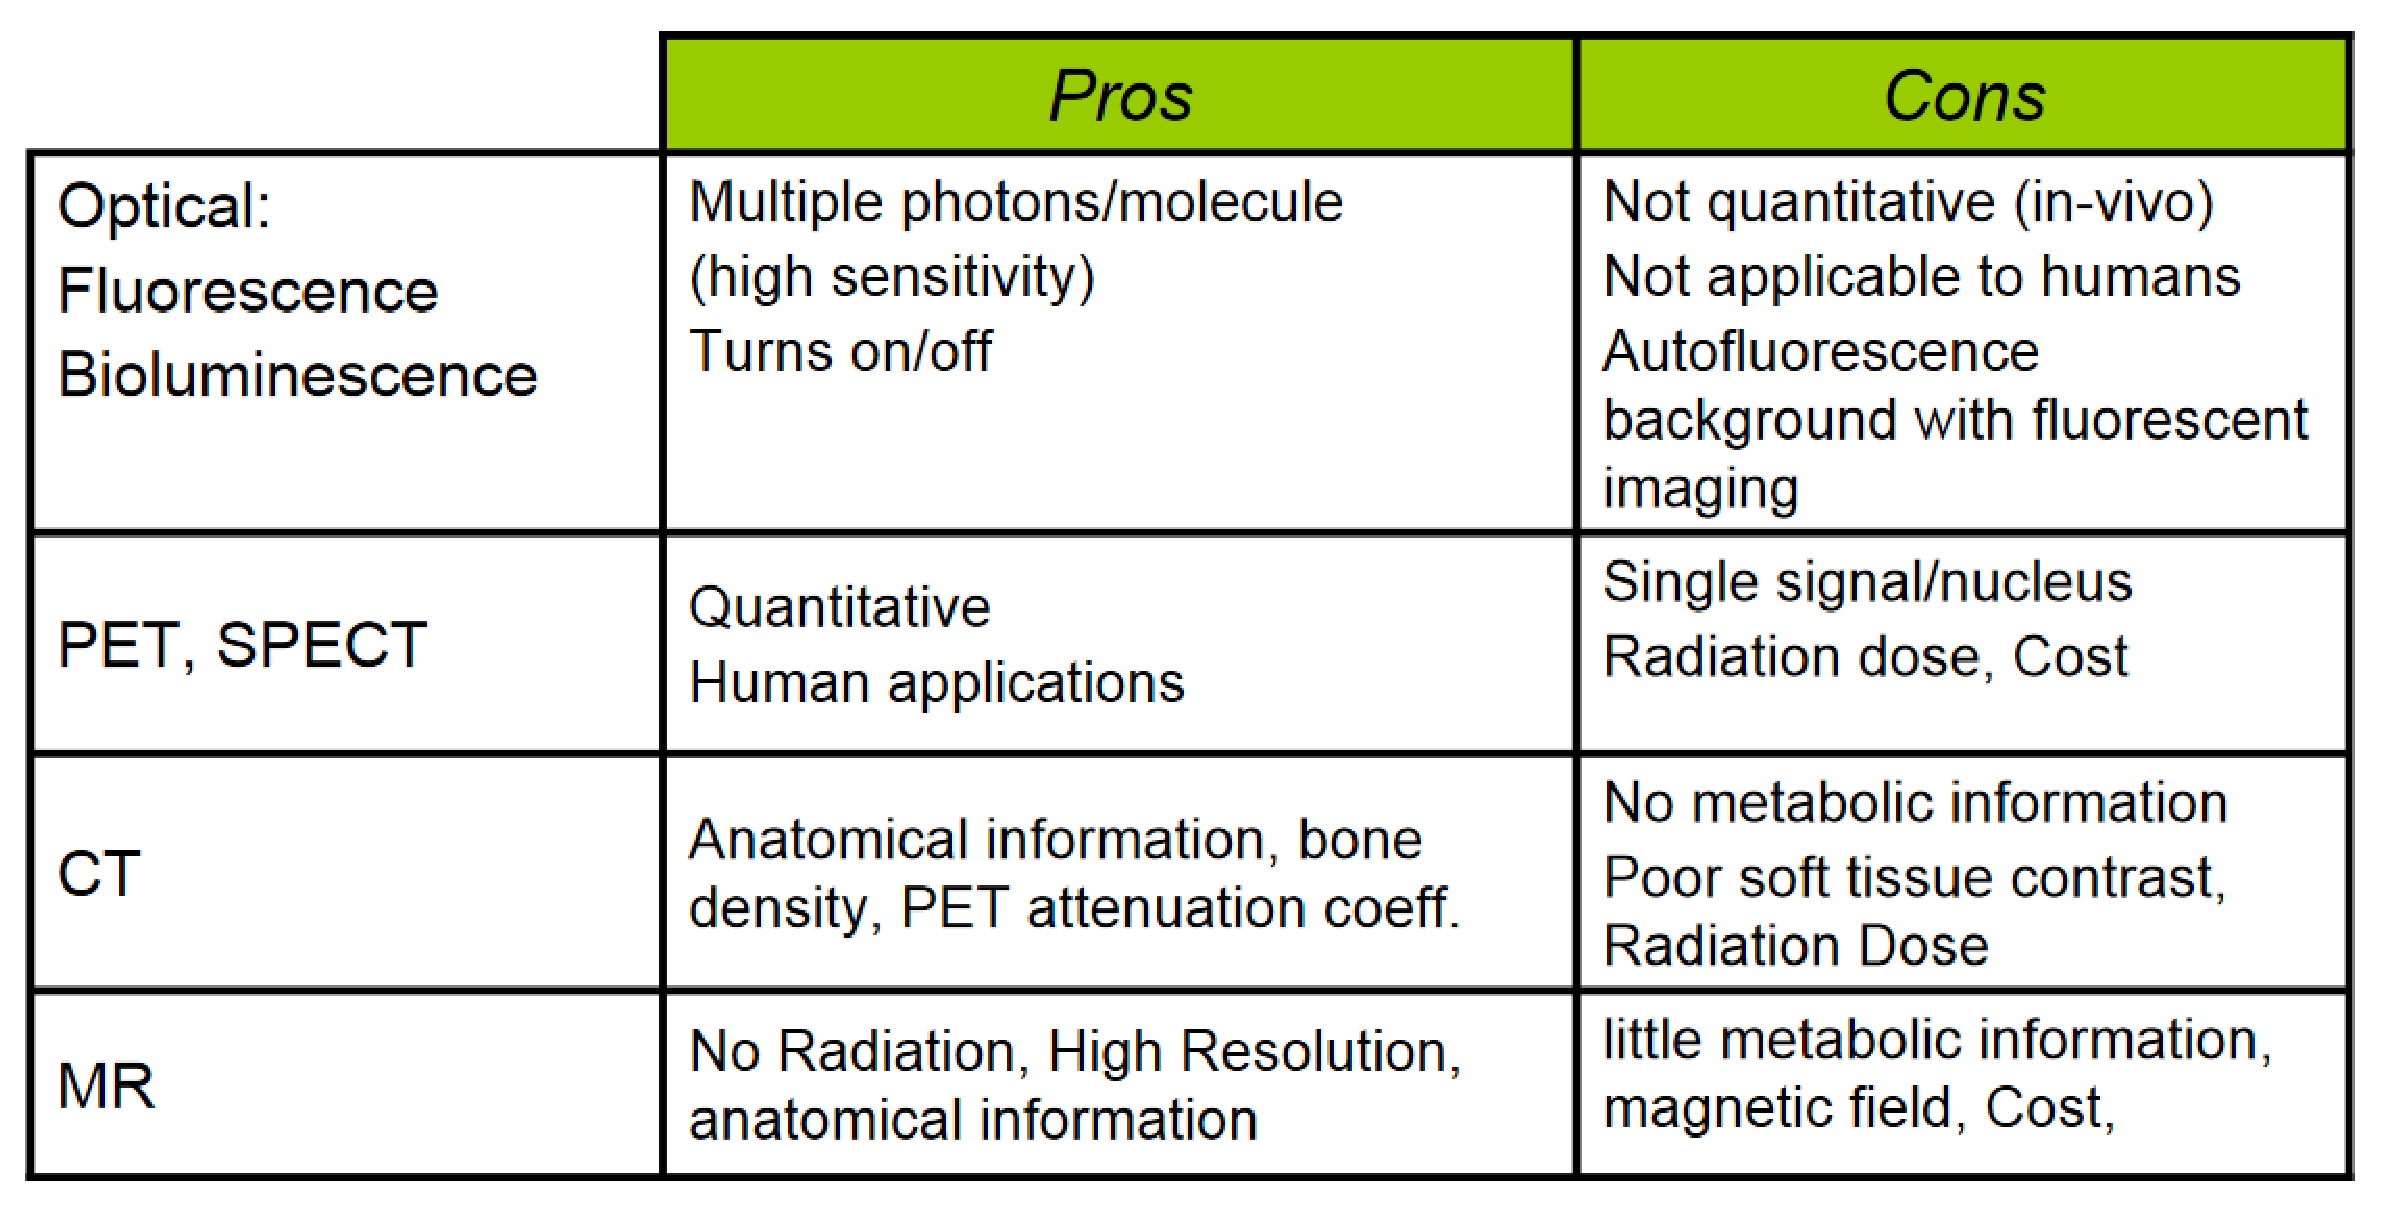
\includegraphics[height=5cm,
    angle=0]{./images/preclincal-imaging-pros-cons.eps}}
\caption{Pros and Const of different imaging techniques}
%http://snmmi.files.cms-plus.com/docs/rpsc_SNMclass2.pdf
\label{fig:preclincal-imaging-pros-cons}
\end{figure}

\begin{figure}[hbt]
  \centerline{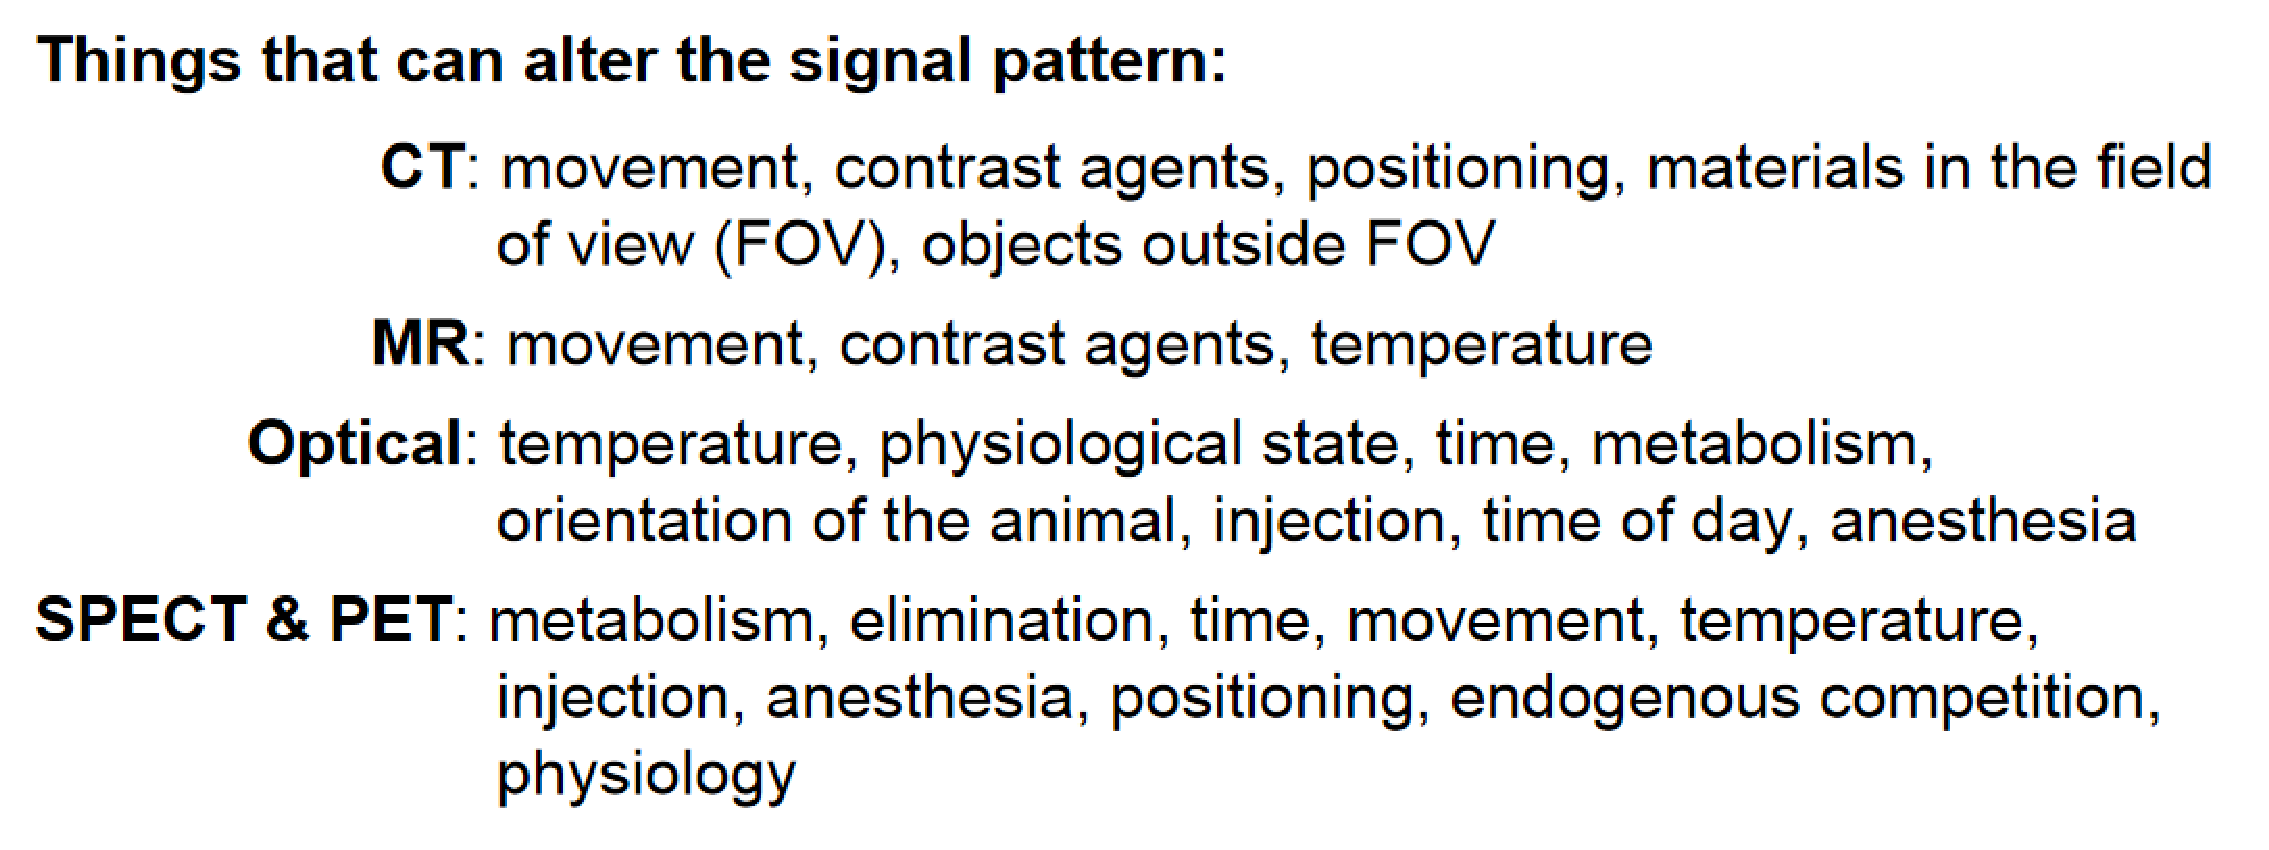
\includegraphics[height=5cm,
    angle=0]{./images/preclincal-imaging-depend.eps}}
\caption{of different imaging techniques}
%http://snmmi.files.cms-plus.com/docs/rpsc_SNMclass2.pdf
\label{fig:preclincal-imaging-depend}
\end{figure}



\url{http://snmmi.files.cms-plus.com/docs/rpsc_SNMclass1.pdf}

\section{PET (positron-emission tomography)}
\label{sec:PET}


The two main functional brain imaging techniques, positron emission tomography
(PET) and functional magnetic resonance imaging (fMRI - Sect.\ref{sec:fMRI}),
detect signals that are directly related to energy delivery and use (Logothetis
et al., 2001; Raichle, 1983, 1998).


The PET scan uses a special dye containing radioactive tracers.
A small amount of liquid radioactive material is injected into the body, either
being swallowed, inhaled, or injected into a vein in your arm depending on what
part of the body is being examined.). Example:
A small needle will be inserted into a vein, usually in your arm or the back of
your hand, to fit an intravenous line (a thin plastic tube) through which the
liquid radioactive material is injected. Your blood sugar level will be checked,
as high or low blood sugar levels can alter the appearance of the scan.
If you are having an FDG-PET scan, you will be asked to rest quietly in a bed or
arm chair, avoiding movement or talking for 90 minutes. During this time you
will be alone. You may be asked to drink some contrast material that moves
through your stomach and bowel, and helps to improve the quality of the images.
Occasionally, depending on the medical condition or symptom, a catheter (a thin
flexible tube) may be placed into your bladder to help improve image quality.
You will then be moved to the scanning room and positioned on the PET scanning
bed. It is important to remain as still as possible during the scan, as movement
can result in reduced image quality and the images may be blurry.
You should drink plenty of fluids after the test is finished. This will flush
the radioactive substance out of the body through the kidneys and into the
bladder. Total time is about 2-3 hours.
The radioactive tracers only remain in your body for a few hours. The radiation
dose you receive is equivalent to several years of natural background radiation
from the normal environment. This small amount of additional radiation does not
cause any side effects.
\url{https://www.insideradiology.com.au/pet-scan/}


IMPORTANT: The radiolabelled molecular probes  have different rates of
uptake depending on the type and function of tissue involved.

\begin{enumerate}

  \item (most common) $^{18}$F or fluorine-18 (F-18) or {\bf  fludeoxyglucose
  ($^{18}$F-labeled 2-deoxyglucose FDG)}, i.e.
  FDG-PET: a simple sugar (like glucose but oxygen atom is replaced by F-18)
  called FDG, which stands for “fluorodeoxyglucose”.

  
  It is injected into the bloodstream and accumulates in the body where it gives
off energy in the form of gamma rays, upon being uptake by glucose-using cells
after that it is phosphorylated by hexokinase (whose mitochondrial form is
greatly elevated in rapidly growing malignant tumors). 
The oxygen atom that is replaced by F-18 to generate FDG is required for the
next step in glucose metabolism in all cells, no further reactions occur in FDG.

   
   NOTE: most tissues (with the notable exception of liver and kidneys) cannot
   remove the phosphate group added (to FDG) by hexokinase. This means that FDG
   is trapped in any cell that takes it up until it decays, since phosphorylated
   sugars, due to their ionic charge, cannot exit from the cell.
   
   This results in intense radiolabeling of tissues with high glucose uptake,
   such as the brain, the liver, and most cancers.


The (high) concentrations of tracer imaged will indicate (high) tissue metabolic
activity as it corresponds to the regional glucose uptake.

The PET scan system detects pairs of gamma rays emitted indirectly by such
positron-emitting radionuclide (tracer). Three-dimensional images of tracer
concentration  within the body are then constructed by computer analysis.
In terms of FDG-PET, the high signal reflects high glucose consumption in
the area, e.g. potentially location of cancer tumors or abnormal high energetic
demand in the brain region.

FDG is also useful for imaging inflammatory or infective processes, and for
imaging brain metabolism (Sect.\ref{sec:PET-neuroimaging}).
  
   \item Less often, other radioactive tracers are used to image the tissue
   concentration of other types of molecules of interest.
   
   \item $^{15}$O$_2$: detect changes in oxygen consumption, which are
   associated with localized brain activities.
   
   \item  $^{15}$O (oxygen-15)-labeled water: reveals changes in cerebral blood flow (CBF)
   
   The blood flow, in general, believed to be correlated, and has been measured
   using the tracer oxygen-15 (with 2-minute half-life). Changing of regional
   blood flow in various anatomic structures (as a measure of the injected
   positron emitter) can be visualized and relatively quantified with a PET scan.
   
   What it measures is actually the flow of blood to different parts of the
   brain. 
   
   \item Detect endocanabinoid system change
   \url{https://link.springer.com/chapter/10.1007/978-3-642-42014-6_11}
    
   
\end{enumerate}

\label{sec:PET-CT-scan}
PET scanners are combined with computed tomography (CT) scanners, called PET-CT
scanners. CT imaging uses X-ray equipment to create detailed images of slices of
the inside of your body. The PET-CT combination allows any abnormality on the
PET scan to be precisely located within the body, allowing for more accurate
diagnosis of any problems. The PET or PET-CT scanner looks like a large box with
a circular hole in the middle.

If you are having a combined PET-CT, the CT scan is done first and takes less than 2
minutes. The PET scan takes approximately 15–20 minutes, but the time will vary
depending on the areas of your body being scanned.


\subsection{PET neuroimaging}
\label{sec:PET-neuroimaging}

{\bf PET neuroimaging}, using FDG-PET, is based on an assumption that areas
   of high radioactivity are associated with brain activity.
   
   
   NOTE: As Alzheimer brain greately decrease brain metabolism of both glucose
   and oxygen in tandem; standard FDG-PET of the brain, which measures regional
   glucose use, may also be successfully used to differentiate Alzheimer's
   disease from other dementing processes.
   
NOTE: In human, the spatial resolution of state-of-the-art PET scanner is 4-6mm;
while in small animal, we expects it to be sub-milimeter. The
photomultiplier-based detector ring diameter for microPET is of approximately
150 mm (6 in), as compared with approximately 800 mm (31 in) for human PET
systems. An exception with LabPET (Gamma Medica/GE Healthcare), which uses
semiconductor avalanche photodiode-based detectors.



\subsection{PET-tau scan}
\label{sec:PET-tau-scan}



\section{microPET (radioisotope distribution) on mice, rat}
\label{sec:microPET}

Small-animal PET refers to imaging of animals such as rats and mice using
dedicated (small, high-resolution) PET scanners and has emerged since 1990s.
Compared with a human PET scanner, a small-animal PET scanner is used for
subjects that typically are 2 to 3 orders less in weight and volume than a
human. NOTE: In human, the spatial resolution of state-of-the-art PET scanner is
4-6mm; while in small animal, we expects it to be sub-milimeter which gives it
the name {\it micro}PET.
When micro is used as a prefix to an imaging modality, such as micro-CT and
micro-MRI, it indicates small-animal imaging.

\begin{mdframed}
The primary use of animal PET is concentrated in
academic  or  government  research  laboratories  (70\%-
80\%), with the remainder being in pharmaceutical and bio-pharmaceutical
companies. PRICE: \$400K to \$1.2M.

Like clinical PET scanners, small-animal PET systems implement 3-dimensional
data acquisition in list mode to enable image time framing and provide
physiologic gating inputs to correct for cardiac and respiratory motion
\end{mdframed}

Developing methods for in vivo molecular imaging in small animals is important
in biomedical research.
\begin{itemize}
  \item  nanoScan PET/MRI and a nanoScan PET/CT (Mediso ltd, Hungary) scanner
  (Nagy et al., 2013)

%   Nagy, K., Toth, M., Major, P., Patay, G., Egri, G., Haggkvist, J., Varrone,
%   A., Farde, L., Halldin, C., and Gulyas, B.
% (2013). Performance evaluation of the small-animal nanoScan PET/MRI system.
% Journal of nuclear medicine : official publication, Society of Nuclear Medicine
% 54, 1825-1832.
  
\end{itemize}

With radiotracer concentrations to be determined in vivo, a dedicated animal
scanner permits the entire time course of a tracer to be measured in a single
animal and provides the means for repeated studies of that same subject over an
arbitrary period of time.
\begin{itemize}
  \item mouse is anesthetized with inhalation of isoflurane and oxygen gases
  
As animals are not cooperated like human, to remain stills during the imaging
(tens of minutes), anesthesia must be used.
NOTE: Because of their smaller bodies, the physiologic conditions of mice and
rats are more susceptible to environmental changes and hypothermia during the
imaging process.
To warrant the reliability and reproducibility of PET data, especially when
physiologic parameters such as blood flow, substrate metabolism, or organ
functions are being investigated, a heating source (light bulb, air flow, or
pad) must be used to maintain the animal's body temperature, and vital signs
must be monitored to verify the animal's homeostasis.

To ensure cons istency during a longitudinal study, certain devices are commonly
used to hold the animals in selected positions.

  \item then, a cannula was inserted in the tail through which the radioligand
  was administered iv.
  \item example, the mouse was imaged with both the dopamine D2
  receptor ligand [11C]raclopride and with [18F]MNI-659, a radioligand for
  imaging of the PDE10A enzyme. 
  
  \item image data files were reconstructed and the individual PET images were
  co-registered to a MRI template in PMOD 3.4 (Zurich, Switzerland)
  
  \item Binding Potential (BPND) in the whole striatum including caudate and putamen was
calculated with the simplified reference tissue method and using the cerebellum
as reference region.
\end{itemize}

There are many different isotopes, with different half-lifes, max energy,
$\beta+$ fraction, and positron ranges. The most widely used isotopes for PET
imaging are F-18, C-11, O- 15 and N-13. The isotope for a particular target is
injected at the tail of the mice.
\begin{enumerate}
  \item PDE10 PET imaging using PDE10 PET ligand [18F]MNI-659 in vivo
  
In vitro: PDE10-selective radioligand \ce{[^3H]-PF-04831704} and PF-06327104.

\end{enumerate}

\begin{figure}[hbt]
  \centerline{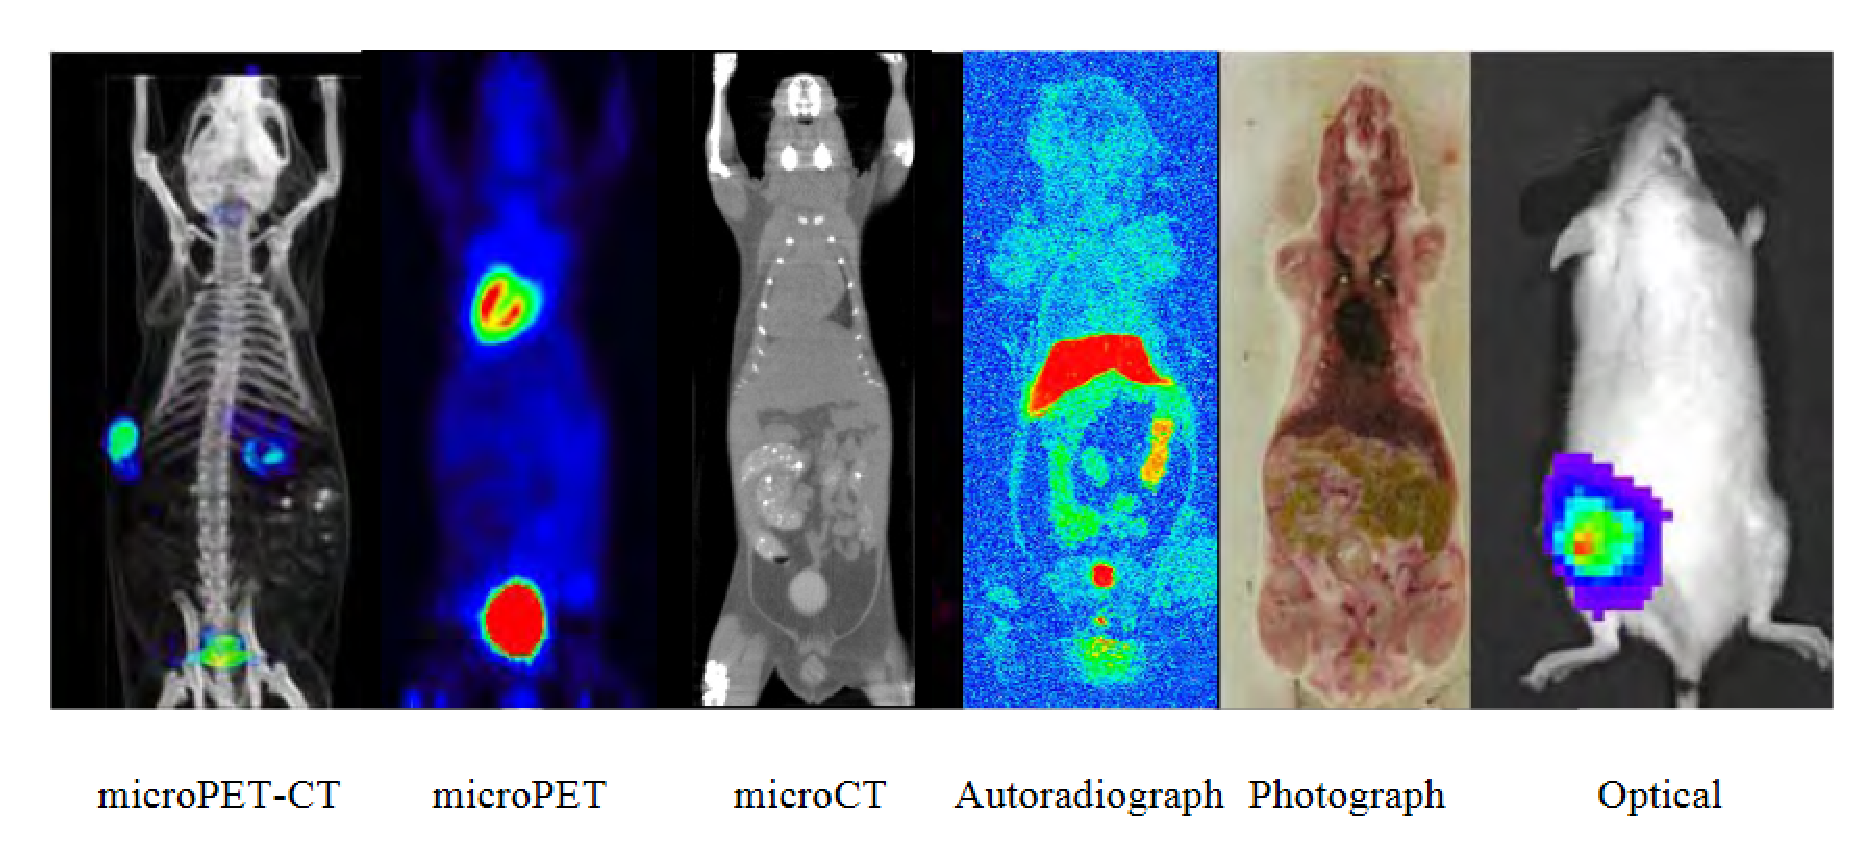
\includegraphics[height=5cm,
    angle=0]{./images/preclincal-imaging.eps}}
\caption{Different imaging techniques}
%http://snmmi.files.cms-plus.com/docs/rpsc_SNMclass1.pdf
\label{fig:preclincal-imaging}
\end{figure}


Example: On the experimental day, mice were anesthetized with inhalation of
isoflurane and a cannula was inserted in the tail through which the radioligand
was administered iv. All PET measurements were performed with a nanoScan
PET/MRI and a nanoScan PET/CT (Mediso ltd, Hungary) scanner (Nagy et al.,
2013). Each mouse was imaged with both the dopamine D2 receptor ligand
[11C]raclopride (Sect.\ref{sec:D2-like-receptors}) and with [18F]MNI-659, a
radioligand for imaging of the PDE10A enzyme (Sect.\ref{sec:PDE10-ligand}).

\begin{mdframed}
\label{sec:binding-potential}

Binding potential (BP) is a combined measure of the density of "available"
neuroreceptors and the affinity of a drug to that neuroreceptor.
So, it is not the exact indicator of neuroreceptor density, as the same density,
but if the affinity change, it still gives a different BP.

Example: A Ligand with a concentration L associates with a receptor of
concentration or availability R to form a ligand-receptor complex with concentration RL.
The BD is the ratio of the complex RL to free ligand at equilibrium and in the
limit $L \rightarrow 0$.
\begin{equation}
\text{BP}_{\text{ND}} = \frac{\text{RL}}{\text{L}}|_{\text{L}\rightarrow 0}
\end{equation}


\url{https://en.wikipedia.org/wiki/Binding_potential}
\end{mdframed}

Binding Potential (BP$_{\text{ND}}$) in the whole striatum including caudate and
putamen was calculated with the simplified reference tissue method and using the
cerebellum as reference region. The difference between WT and Q175 was analyzed
with Student t-test (p-value <0.05 was considered significant). PET images are
displayed as standard uptake value (SUV\% = kBq/cc $\div$ MBq injected / body
weight (g) * 100).


\section{Optical method (light making it out of the body)}

Chap.\ref{chap:Imaging_Tech}.
\begin{itemize}
  \item Bioluminescent Imaging: Light generated within animal, emitted and detected

  \item Fluorescent Imaging: Light shined on animal, fluorophore wave shifts the light, 
light travels back out for detection
\end{itemize}

However, the data is not quantitative (in-vivo); and not applicable to humans.


\section{MR (proton density)}
\section{microCT (electron density)}
\label{sec:microCT}

A typical microCT system can produce images of 50 micron resolution ($\approx$ 25
micron pixel size) or greater.
High resolution is only possible in ex vivo imaging protocols, since heart and
respirator movement will blur in vivo images.

Unlike human CT scanners, most preclinical CT systems required several 
minutes to acquire data, thus conventional CT contrast agents that last 2-3 
seconds are not suitable.

Recently longer lasting liver \& vascular CT contrast agent Fenestra has been
developed.



